% ----- Internal helper (now uses #1...#8 correctly) -----
\newcommand{\event}[8]{%
    \pgfmathsetmacro{\x}{(#1 - \timelineStart) * \timelineScale}%
    \pgfmathsetmacro{\y}{#6}%
    \begin{scope}[on background layer]
        \draw[thick, dashed] (\x,0) -- ++(0,\y);
    \end{scope}
    \node[
        draw, rounded corners, very thick, fill=#8,
        minimum height=#5, text width=#4, align=center, font=#7
    ] at (\x,\y) {\textbf{\cite{#2}} \\[2pt] #3};
}

% ----- Main timeline command -----
% Usage: \Timeline[start_year,end_year,scale]{ list of \event{...} ... }
\newcommand{\Timeline}[2][1943,2025,0.3]{%
    % Extract parameters
    \edef\timelineParams{#1}%
    \pgfmathsetmacro{\timelineStart}{{\timelineParams}[0]}%
    \pgfmathsetmacro{\timelineEnd}{{\timelineParams}[1]}%
    \pgfmathsetmacro{\timelineScale}{{\timelineParams}[2]}%
    %
    \begin{tikzpicture}
        % Main timeline arrow
        \draw[draw, thick, -{Stealth[length=3mm]}, line cap=round] 
            (0,0) -- ({(\timelineEnd - \timelineStart) * \timelineScale},0);
        % All events
        #2
    \end{tikzpicture}%
}
\newif\ifdraftfigures

\newcommand{\heavyfig}[2]{%  #1 = label to preserve, #2 = figure file
    \ifdraftfigures
        \begin{figure}[t]
            \centering
            \fbox{\parbox[c][3cm][c]{0.6\linewidth}{\centering\itshape
                Heavy figure skipped in draft mode}}
            \caption{\itshape Figure skipped in draft mode
                (set \texttt{\string\draftfiguresfalse} to render it).}
            \label{#1}
        \end{figure}%
    \else
        \input{#2}%
    \fi
}

\AddToShipoutPictureBG{%
    \AtPageLowerLeft{%
        \hspace{\dimexpr\oddsidemargin+1in\relax}%
        \raisebox{0.8cm}{%
            \parbox{\textwidth}{%
                \centering\color{gray}
                Compiled on \the\day/\the\month/\the\year\ at \currenttime
            }%
        }%
    }%
}

\tcbset{
  mydefinition/.style={
    colback=gray!5,
    colframe=gray!60,
    boxrule=0.5pt,
    arc=3pt,
    left=6pt,
    right=6pt,
    top=4pt,
    bottom=6pt,
    fonttitle=\bfseries,
    coltitle=black
  }
}

\newtcbtheorem[number within=section]{definition}{Definition}{
  mydefinition
}{def}

\tcbset{
  myhypothesis/.style={
    colback=orange!5,
    colframe=orange!70!black,
    boxrule=0.5pt,
    arc=3pt,
    left=6pt,
    right=6pt,
    top=4pt,
    bottom=6pt,
    fonttitle=\bfseries,
    coltitle=black
  }
}

\newtcbtheorem{hypothesis}{Hypothesis}{
  myhypothesis
}{hyp}

% Defined here, before \newacronym below, since the CU/AS/ACU acronym
% descriptions reference these macros directly.
\newcommand{\BehaviorReconstructionName}{\textit{Behavior Reconstruction}\xspace}
\newcommand{\ClusteringUniversalityName}{\textit{Clustering Universality}\xspace}
\newcommand{\AbstractionScoreName}{\textit{Abstraction Score}\xspace}
\newcommand{\AdjustedClusteringUniversalityName}{\textit{Adjusted Clustering Universality}\xspace}

\makeglossaries
\setglossarystyle{index}
\setabbreviationstyle[acronym]{long-short}
\newacronym{ai}{AI}{Artificial Intelligence}
\newacronym{rl}{RL}{Reinforcement Learning}
\newacronym{xai}{XAI}{eXplainable Artificial Intelligence}
\newacronym{xrl}{XRL}{eXplainable Reinforcement Learning}
\newacronym{dl}{DL}{Deep Learning}
\newacronym{nn}{NN}{Neural Network}
\newacronym{ls}{LS}{Latent Space}
\newacronym{lr}{LR}{Latent Representation}
\newacronym{cs}{CS}{Concept Structure}
\newacronym{llm}{LLM}{Large Language Model}
\newacronym{car}{CAR}{Clustering Agent Representation}
\newacronym{me}{ME}{Mechanistic Explainability}
\newacronym{mlp}{MLP}{MultiLayer Perceptron}
\newacronym{cnn}{CNN}{Convolutional Neural Network}
\newacronym{lstm}{LSTM}{Long Short-Term Memory}
\newacronym{sgd}{SGD}{Stochastic Gradient Descent}
\newacronym{sae}{SAE}{Sparse Autoencoder}
\newacronym{mse}{MSE}{Mean Squared Error}
\newacronym{dqn}{DQN}{Deep Q-Networks}
\newacronym{ddpg}{DDPG}{Deep Deterministic Policy Gradient}

\newacronym{ppo}{PPO}{Proximal Policy Optimization}
\newacronym{appo}{APPO}{Asynchronous Proximal Policy Optimization}
\newacronym{mdp}{MDP}{Markov Decision Processes}
\newacronym{ari}{ARI}{Adjusted Rand Index}
\newacronym{ri}{RI}{Rand Index}
\newacronym{cu}{CU}{\ClusteringUniversalityName}
\newacronym{as}{AS}{\AbstractionScoreName}
\newacronym{acu}{ACU}{\AdjustedClusteringUniversalityName}
\newacronym{gmm}{GMM}{Gaussian Mixture Model}
\newacronym{bc}{BC}{Behavioral Cloning}

\newacronym{gpu}{GPU}{Graphics Processing Unit}
\newacronym{cpu}{CPU}{Central Processing Unit}
\newacronym{hpc}{HPC}{High-Performance Computing}
\newacronym{api}{API}{Application Programming Interface}

\colorlet{myred}{red!60!black}
\colorlet{mygreen}{green!50!black}
\colorlet{myblue}{blue!80!black}

% PlotNeuralNet layer colors, kept consistent with the encoder/policy accents
% used in the clustering agent representation figures.
\colorlet{ObservationColor}{black!10!white}
\colorlet{ConvColor}{myblue!35!white}
\colorlet{FcColor}{black!12!white}
\colorlet{FlattenColor}{mygreen!12!white}
\colorlet{OutputColor}{myred!45!white}
\tikzset{connection/.style={ultra thick, every node/.style={sloped, allow upside down}, draw=\edgecolor, opacity=0.7}}

\newcommand{\methodName}{Clustering Agent Representation\xspace}
\newcommand{\emphasize}[1]{\textbf{#1}}

\newcommand{\ConceptHypothesisName}{\textit{Concept Hypothesis}~(Hyp.~\ref{hyp:concept})\xspace}
\newcommand{\SuperpositionHypothesisName}{\textit{Superposition Hypothesis}~(Hyp.~\ref{hyp:superposition})\xspace}
\newcommand{\MechanisticHypothesisName}{\textit{Mechanistic Hypothesis}~(Hyp.~\ref{hyp:mechanistic})\xspace}
\newcommand{\RepresentationConvergenceHypothesisName}{\textit{Representation Convergence  Hypothesis}~(Hyp.~\ref{hyp:convergence})\xspace}



% Reinforcement learning notation: state sets and states
\newcommand{\StateSet}{\mathcal{S}}
\newcommand{\StateSetInitial}{\mathcal{S}^{\text{init}}}
\newcommand{\StateSetTerminal}{\mathcal{S}^{\text{ter}}}
\newcommand{\StateInitial}{s^{\text{init}}}
\newcommand{\StateTerminal}{s^{\text{ter}}}

\newcommand{\InitialPolicy}{\textcolor{mygreen}{\pi}}
\newcommand{\SurrogatePolicy}[1]{\textcolor{myred}{\pi'_{#1}}}

% Deep learning notation: per-example loss
% #1 = parameters (\theta, \theta^{(n)}, ...), #2 = training-example index
\newcommand{\fullLoss}[2]{\mathcal{L}\left(\hat{f}_{#1}(x^{(#2)}), y^{(#2)}\right)}
\newcommand{\loss}[2]{\mathcal{L}^{(#2)}\left(#1\right)}

% Deep learning notation: latent representation (\gls{lr})
% Optional #1 = layer index; \latentRepresentation -> h, \latentRepresentation[l] -> h_{l}
\newcommand{\latentRepresentation}[1][]{%
    \mathbf{h}\if\relax\detokenize{#1}\relax\else_{#1}\fi
}

% Environment names, used every time one of the six Atari games is named in
% the text or in a figure, so their formatting (bold) stays consistent.
\newcommand{\BreakoutName}{\textbf{Breakout}\xspace}
\newcommand{\MarioBrosName}{\textbf{Mario Bros}\xspace}
\newcommand{\MsPacManName}{\textbf{Ms.\ Pac-Man}\xspace}
\newcommand{\PongName}{\textbf{Pong}\xspace}
\newcommand{\SpaceInvadersName}{\textbf{Space Invaders}\xspace}
\newcommand{\SurroundName}{\textbf{Surround}\xspace}

\definecolor{spaceInvadersColor}{RGB}{0, 0, 255}
\newcommand{\spaceInvadersMark}{*}
\newcommand{\spaceInvadersMarkSize}{0.06cm}

\definecolor{marioBrosColor}{RGB}{255, 0, 0}
\newcommand{\marioBrosMark}{square*}
\newcommand{\marioBrosMarkSize}{0.05cm}

\definecolor{pongColor}{RGB}{255, 192, 203}
\newcommand{\pongMark}{x}
\newcommand{\pongMarkSize}{0.11cm}

\definecolor{breakoutColor}{RGB}{0, 127, 0}
\newcommand{\breakoutMark}{triangle*}
\newcommand{\breakoutMarkSize}{0.08cm}

\definecolor{surroundColor}{RGB}{255, 165, 0}
\newcommand{\surroundMark}{diamond*}
\newcommand{\surroundMarkSize}{0.1cm}

\definecolor{msPacmanColor}{RGB}{148, 0, 211}
\newcommand{\msPacmanMark}{pentagon*}
\newcommand{\msPacmanMarkSize}{0.06cm}

\def\numberOfSamplesToPlotCurve{50}
% define gaussian pdf
\pgfmathdeclarefunction{gauss}{3}{%
  \pgfmathparse{1/(#3*sqrt(2*pi))*exp(-((#1-#2)^2)/(2*#3^2))}%
}


% Compact float layout, meant for the Experiments chapter only (see
% chapters/experiments/experiments.tex): up to 6 floats per page, tighter
% spacing. Everywhere else the strict layout of packages.tex applies (one
% float per page, at the top). \DisableCompactFloats restores it, saving the
% skips first so that the values in force before are put back exactly.
\newskip\savedfloatsep
\newskip\savedtextfloatsep
\newskip\savedintextsep
\newlength\savedabovecaptionskip
\newlength\savedbelowcaptionskip
\newcommand{\EnableCompactFloats}{%
  \FloatBarrier
  \setlength{\savedfloatsep}{\floatsep}%
  \setlength{\savedtextfloatsep}{\textfloatsep}%
  \setlength{\savedintextsep}{\intextsep}%
  \setlength{\savedabovecaptionskip}{\abovecaptionskip}%
  \setlength{\savedbelowcaptionskip}{\belowcaptionskip}%
  \setcounter{topnumber}{6}%
  \setcounter{bottomnumber}{6}%
  \setcounter{totalnumber}{6}%
  \renewcommand{\topfraction}{0.98}%
  \renewcommand{\bottomfraction}{0.98}%
  \renewcommand{\textfraction}{0.02}%
  \renewcommand{\floatpagefraction}{0.3}%
  \setlength{\floatsep}{4pt plus 1pt minus 1pt}%
  \setlength{\textfloatsep}{6pt plus 1pt minus 1pt}%
  \setlength{\intextsep}{4pt plus 1pt minus 1pt}%
  \setlength{\abovecaptionskip}{3pt}%
  \setlength{\belowcaptionskip}{3pt}%
}
\newcommand{\DisableCompactFloats}{%
  \FloatBarrier
  \setcounter{topnumber}{1}%
  \setcounter{bottomnumber}{0}%
  \setcounter{totalnumber}{1}%
  \renewcommand{\topfraction}{0.9}%
  \renewcommand{\bottomfraction}{0.3}%
  \renewcommand{\textfraction}{0.1}%
  \renewcommand{\floatpagefraction}{0.5}%
  \setlength{\floatsep}{\savedfloatsep}%
  \setlength{\textfloatsep}{\savedtextfloatsep}%
  \setlength{\intextsep}{\savedintextsep}%
  \setlength{\abovecaptionskip}{\savedabovecaptionskip}%
  \setlength{\belowcaptionskip}{\savedbelowcaptionskip}%
}

% ---------------------------------------------------------------------------
% Shared building blocks for the metric-vs-K tables of Appendix~\ref{chap:appendix}
% (see appendix/additional_results/additional_results.tex and
% tables/additional_results/*.tex), factored out so every table only needs to
% supply its data.
% ---------------------------------------------------------------------------

% ---------------------------------------------------------------------------
% Core of the metric-vs-K tables of Appendix~\ref{chap:appendix}: cell macros
% and the table body itself. Kept in its own file because it is shared by
% setup.tex (live typesetting) and by build_tables.tex, which compiles every
% table once into tables/additional_results/tables.pdf (see setup.tex).
% Only relies on xcolor (with \myblue), tabularray, diagbox, amsmath.
% ---------------------------------------------------------------------------

% Maximum tint (percent) of the heatmap at value = 1; kept low enough that
% black text stays legible on top of it.
\newcommand{\HeatCellMaxPct}{55}
% Cell padding: how much horizontal/vertical room surrounds each cell's
% content. Tune these two to change the width/height of every cell at once.
\newcommand{\ClusterKTableColSep}{1.2pt}
\newcommand{\ClusterKTableRowSep}{1.5pt}
% Tables with more rows (8 layers, i.e. 10 rows) get a tighter row padding so
% that their natural aspect ratio comes close to that of the shorter ones:
% every table then ends up with the same size and font scale in the same box.
\newcommand{\ClusterKTableRowSepTall}{0.6pt}
% Thickness of the rules separating the header / data / aggregate zones.
\newcommand{\ClusterKTableZoneRule}{1pt}

% #1 = condition (0 or 1), #2 = one-argument wrapping macro, #3 = content
\newcommand{\wrapif}[3]{\ifnum#1=1 #2{#3}\else#3\fi}

% The text of a data cell -- #1 = value, #2 = is column-best (0/1), #3 = is
% row-best (0/1). Its background is set separately by \SetCell right before
% it (tabularray requires \SetCell to appear literally first in the cell, so
% it cannot be hidden inside this macro) -- see the heatmap computation
% below, done live in LaTeX via \numexpr from the raw value.
\newcommand{\CellText}[3]{\wrapif{#2}{\textbf}{\wrapif{#3}{\underline}{#1}}}

% Background key for a data cell, e.g. \SetCell{bg=\HeatCellBg{97}} -- #1 is
% the value scaled to an integer in hundredths (97 for 0.97, -22 for -0.22);
% the tint percentage is computed live from it via integer arithmetic
% (\numexpr), clamped to 0 below zero since only non-negative values are
% tinted.
\newcommand{\HeatCellBg}[1]{myblue!\ifnum#1>0 \the\numexpr(#1*\HeatCellMaxPct/100)\relax\else0\fi}

% An aggregate "mean $\pm$ std" cell -- #1 = mean, #2 = std, #3 = is the best
% mean of the aggregate row/column (0/1).
\newcommand{\MeanCell}[3]{\wrapif{#3}{\textbf}{#1} $\pm$\,#2}

% The table itself -- #1 = index of the last (Mean +- Std) row, #2 = data rows
% (including the trailing Mean +- Std row).
\newcommand{\ClusterKTableBody}[2]{%
  {\scriptsize
  \begin{tblr}{
    colspec={|c|*{19}{c|}c|},
    colsep=\ClusterKTableColSep,
    rowsep=\ifnum#1>8 \ClusterKTableRowSepTall\else\ClusterKTableRowSep\fi,
    hlines,
    vlines,
    hline{2} = {\ClusterKTableZoneRule},
    hline{#1} = {\ClusterKTableZoneRule},
    vline{2} = {\ClusterKTableZoneRule},
    vline{21} = {\ClusterKTableZoneRule},
    row{1} = {font=\bfseries, halign=c, valign=m},
    column{1} = {halign=c, valign=m},
    row{#1} = {font=\itshape},
    column{21} = {font=\itshape},
  }
  \diagbox[width=5em,height=2.8em,innerleftsep=1pt,innerrightsep=1pt]{\scriptsize Layer}{\scriptsize $K$} & 2 & 3 & 4 & 5 & 6 & 7 & 8 & 9 & 10 & 11 & 12 & 13 & 14 & 15 & 16 & 17 & 18 & 19 & 20 & Mean $\pm$ Std \\
  #2
  \end{tblr}%
  }%
}


% Vertical budget of the metric-vs-K tables, so that each environment of the
% appendix fits on \ClusterKTablesPerPage tables per (landscape) page, i.e. two
% pages for the six tables of an environment. Every table is scaled to fill
% the full line width and this height:
%   (\textheight - heading allowance) / tables per page - caption overhead,
% \textheight being the landscape height when used inside the landscape
% environment. If the tables come out too small, lower the two allowances; if
% an environment still spills onto a third page, raise them.
\newcommand{\ClusterKTablesPerPage}{3}
% Room taken by the section heading on the first page of an environment.
\newcommand{\ClusterKTableHeadingAllowance}{45pt}
% Caption line plus the spacing around one table.
\newcommand{\ClusterKTableCaptionOverhead}{32pt}
\newlength{\ClusterKTableMaxHeight}
\newsavebox{\ClusterKTableBox}

% Typesetting these tables with tabularray is very slow (about 200 cells each,
% 36 tables), so each one is compiled only once, by build_tables.sh, into one
% page of tables/additional_results/tables.pdf, and the page number is recorded
% in tables/additional_results/tables_pages.tex. \ClusterKTable then merely
% includes that page. A table missing from that file (e.g. one just added) is
% typeset live instead, so nothing breaks before the next build. Re-run
% build_tables.sh whenever the data of a table or the core file changes.
\InputIfFileExists{tables/additional_results/tables_pages.tex}{}{}

% Shared skeleton of a metric-vs-K table -- #1 = index of the last (Mean +-
% Std) row, #2 = caption, #3 = label suffix, #4 = data rows (including the
% trailing Mean +- Std row). In draft mode (\draftfigurestrue) a placeholder
% keeping the caption and label is emitted instead of the table.
\newcommand{\ClusterKTable}[4]{%
  \ifdraftfigures
  \begin{table}[H]
  \centering
  \fbox{\parbox[c][3cm][c]{0.6\linewidth}{\centering\itshape
    Heavy table skipped in draft mode}}
  \caption{#2}
  \label{tab:appendix_additional_results_#3}
  \end{table}
  \else
  \begin{table}[H]
  \centering
  \setlength{\ClusterKTableMaxHeight}{\dimexpr(\textheight-\ClusterKTableHeadingAllowance)/\ClusterKTablesPerPage-\ClusterKTableCaptionOverhead\relax}%
  \ifcsname ClusterKPage@#3\endcsname
  \edef\ClusterKCurrentPage{\csname ClusterKPage@#3\endcsname}%
  \includegraphics[page=\ClusterKCurrentPage,width=\linewidth,height=\ClusterKTableMaxHeight,keepaspectratio=false]{tables/additional_results/tables.pdf}%
  \else
  \sbox{\ClusterKTableBox}{\ClusterKTableBody{#1}{#4}}%
  \resizebox*{\linewidth}{\ClusterKTableMaxHeight}{\usebox{\ClusterKTableBox}}%
  \fi
  \caption{#2}
  \label{tab:appendix_additional_results_#3}
  \end{table}
  \fi
}